\documentclass[11pt,xcolor=table]{beamer}
\usepackage[utf8]{inputenc}
\usepackage{listings}
\usepackage{color}

\usecolortheme{rose}
\definecolor{color}{HTML}{009900}
\usetheme{Darmstadt}
\setbeamertemplate{navigation symbols}{}
%\setbeamercolor{frametitle}{fg=white}
\setbeamercolor{structure}{bg=black, fg=color}

\setbeamertemplate{section in toc}{%
  {\color{orange!70!black}\inserttocsectionnumber.}~\textbf{\inserttocsection}}
\setbeamercolor{section in toc}{fg=black}
\setbeamercolor{subsection in toc}{bg=white,fg=black}
\setbeamercolor{bibliography item}{fg=black}
\setbeamercolor*{bibliography entry author}{fg=black}
\setbeamertemplate{subsection in toc}{%
  \hspace{1.2em}{\color{orange}\rule[0.3ex]{3pt}{3pt}}~\inserttocsubsection\par}


\title{Verifica automatica della proprietà di\\ sicurezza forte}

\author{Gianluca Lutero}
\institute{Alma Mater Studiorum Bologna\\Crittografia}
\date{}

\begin{document}

\begin{frame}{}
    \maketitle
\end{frame}

\begin{frame}{Outline}
    \begin{itemize}
        \item Introduzione
        \item Calcolo dei processi
        \item Segretezza forte
        \item Implementazione
        \item Algoritmo di risoluzione
    \end{itemize}
\end{frame}

\begin{frame}{Introduzione}
    far vedere esempio con differenza tra segretezza standard e segretezza forte
\end{frame}

\section{Calcolo dei processi}
\subsection{}
\begin{frame}{Calcolo dei processi}
    \begin{figure}[h]
        \centering
        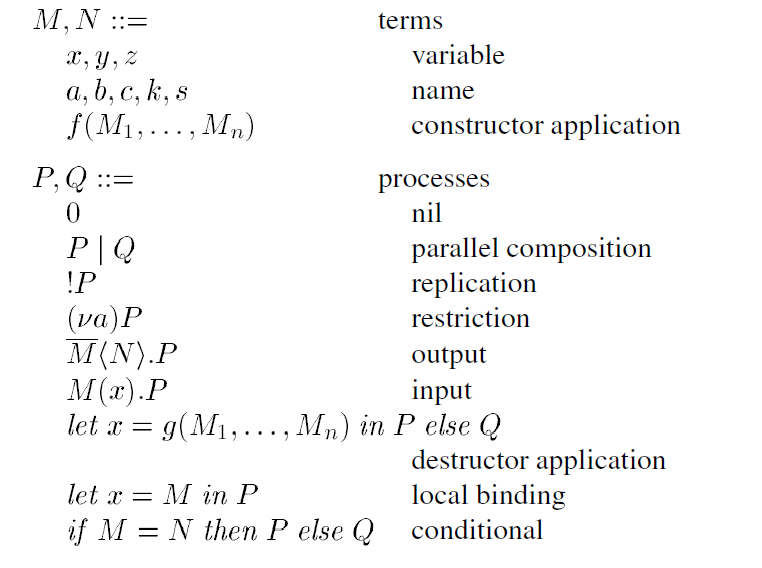
\includegraphics[scale=0.5]{Relazione/Immagini/calcolo.PNG}
    \end{figure}
\end{frame}

\section{Segretezza forte}
\subsection{}
\begin{frame}{Segretezza forte}
    \begin{block}{Segretezza}
        L'avversario non può ottenere il valore del segreto.
    \end{block}
    \vspace{5mm}
    \begin{block}{Segretezza forte}
        Questa proprietà esprime l'impossibilità da parte dell'avversario di sapere quando il valore del segreto cambia.
    \end{block}
\end{frame}

\begin{frame}{Equivalenza osservazionale}
    Si definisce equivalenza osservazionale $\approx$ la piú grande relazione simmetrica $R$ tra processi chiusi tale che $PRQ$ implica:\\
    \begin{enumerate}
        \item se $P \Downarrow m$ allora $Q \Downarrow m$
        \item se $P \rightarrow P'$ allora esiste $Q'$ tale che $Q \rightarrow^* Q'$ e $P'RQ'$
        \item $C[P]RC[Q]$ per tutti i contesti di valutazione chiusi $C$.
    \end{enumerate}
\end{frame}

\begin{frame}{}
    \begin{block}{Proprietà}
        Il processo $P_0$ preserva la segretezza forte delle sue variabili libere se e solo se per ogni sostituzione chiusa $\sigma$ e $\sigma'$ di dominio $fv(P_0)$ , $\sigma P_0 \approx \sigma' P_0$.
    \end{block}
    
    \begin{block}{}
        La proprietà di segretezza forte è vista come un caso particolare di equivalenza osservazionale.
    \end{block}
\end{frame}


\section{Verifica dei protocolli}
\subsection{}
\begin{frame}{Verifica dei protocolli}
    \begin{block}{Termini e fatti}
        I protocolli espressi nel formalismo del calcolo dei processi vengono tradotti in clausole di Horn usando i seguenti termini e fatti
    \end{block}
    \vspace{1cm}
    \begin{columns}
        \begin{column}{0.55\textwidth}
            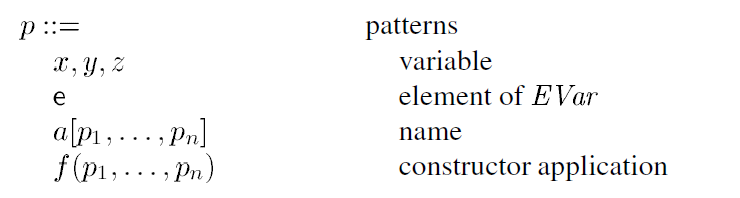
\includegraphics[scale=0.45]{Relazione/Immagini/rule.PNG}
        \end{column}
        
        \begin{column}{0.48\textwidth}
            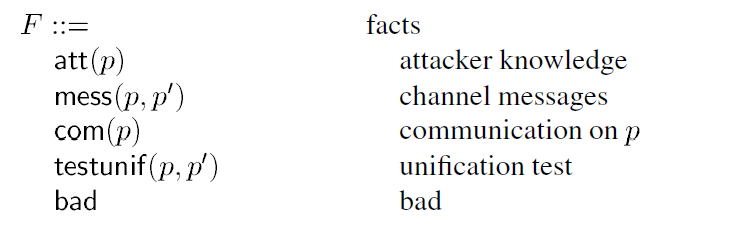
\includegraphics[scale=0.4]{Relazione/Immagini/fatti.PNG}
        \end{column}
    \end{columns}
\end{frame}

\subsection{}
\begin{frame}{Regole}
    \begin{columns}
        \begin{column}{0.55\textwidth}
            Regole per l'avversario\\
            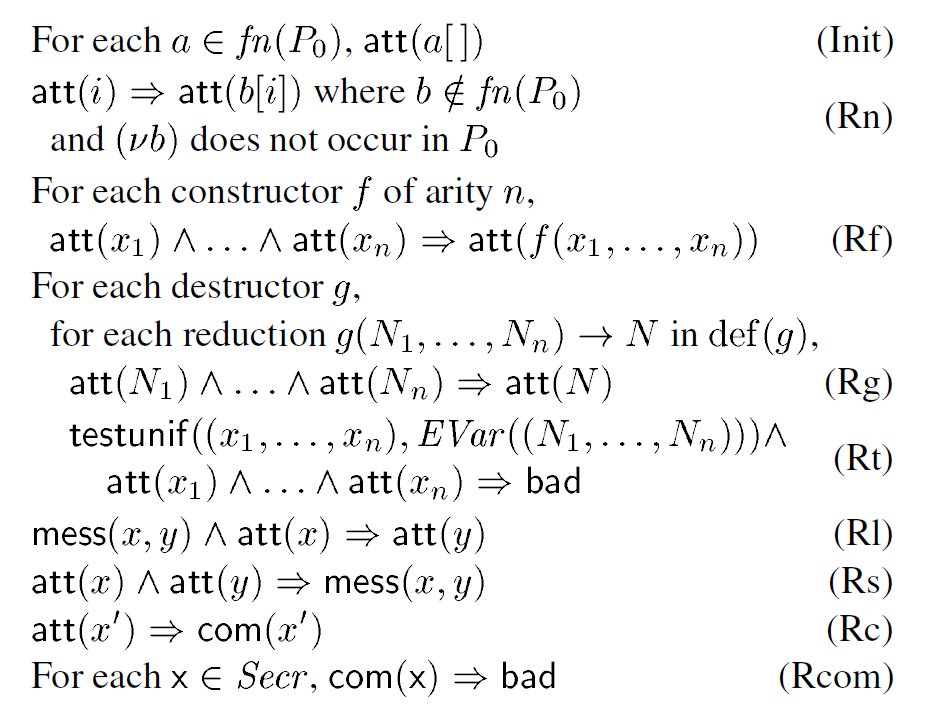
\includegraphics[scale=0.3]{Relazione/Immagini/term_rule.PNG}
        \end{column}
        \begin{column}{0.48\textwidth}
            Regole per i protocolli\\
            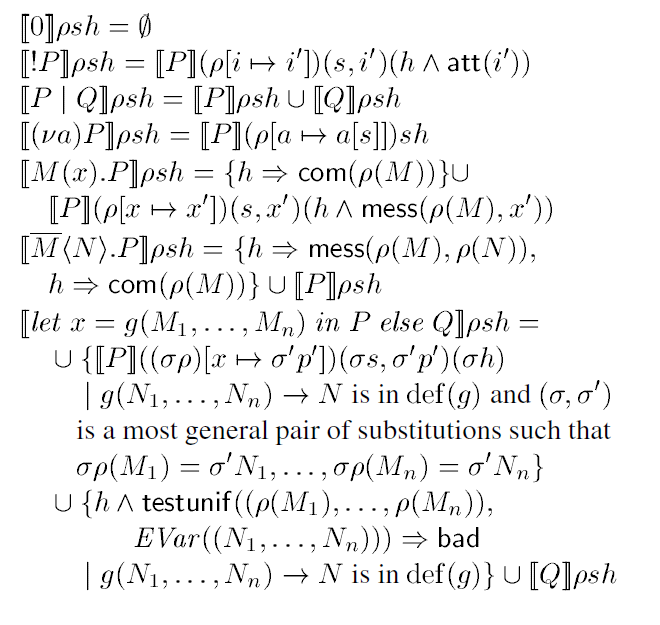
\includegraphics[scale=0.35]{Relazione/Immagini/semantic.PNG}
        \end{column}
    \end{columns}
\end{frame}

\section{Algoritmo di risoluzione}
\subsection{}
\begin{frame}{Algoritmo di risoluzione}
    \begin{block}{}
        Per determinare se un fatto è derivabile da una proposizione si usa la seguente regola:\\
        \begin{center}
            $\frac{H\Rightarrow C \hspace{2cm} F \land H' \Rightarrow C'}{\sigma H \land \sigma H' \Rightarrow \sigma C'}$
        \end{center}
        con C ed F unificabili e $\sigma$ il più generico unificatore per C ed F
    \end{block}
\end{frame}

\subsection{}
\begin{frame}{Funzione di selezione}
    Ogni passo di riduzione è guidato dalla seguente funzione di selezione:\\
    \begin{itemize}
    \item quando la proposizione è \\$R = testunif((x_1),(x_2))\ \land \ att(x_1)\ \land \ att(x_2)\ \Rightarrow \ bad$:\\
    
    $sel(R) = \{att(x_1)\}$
    \item per tutte le altre proposizioni $sel(R)$ è definita come:\\
    
    $
    sel(H\ \Rightarrow \ C)\ =\  
    \begin{cases} 
    \emptyset & \text{se tutti gli elementi di H sono nella forma } \\
    &  att(x) \text{, con x variabile, o testunif(p,p')} \\
    \{F\} & \text{dove } F\ \neq \ att(x), F\ \neq \ testunif(p,p'),\\
    & \text{con } F \in H, \text{ altrimenti}
    \end{cases}
   $
 \end{itemize}
\end{frame}

\subsection{}
\begin{frame}{testunif}
    \begin{block}{Il fatto $testunif$}
        Il predicato $testunif$ è l'unico a non essere definito per mezzo di clausole di Horn.
    \end{block}
    
    \begin{block}{Semplificazione}
    Per valutarne il valore di verità vengono introdotti specifici passi di semplificazione nell'algoritmo di risoluzione. Le semplificazioni effettuate hanno come obiettivo quello di ridurre le dimensione dei fatti $testunif$, progredire verso la conoscenza del valore di verità di questi e semplificarli quando il loro valore di verità è noto.
    \end{block}
\end{frame}

\subsection{}
\begin{frame}{Semplificazione}
    \begin{block}{}
        I passi di semplificazione che possono essere effettuati sono riassunti dalla funzione 
            $simplify\ =\ elimtaut\ \circ \ elimattx\ \circ \ simptestuniftrue\ \circ \ simptestuniffalse\ \circ \ repeat(elimvar\ \circ \ instantiate\ \circ \ elimEVar\ \circ \ swap\ \circ \ unify) $
        
    \end{block}
    
    \begin{block}{}
        L'algoritmo genera la proposizione $bad$ se e solo se $bad$ è derivabile dalle regole del processo. Quindi se non viene generato $bad$ il processo preserva la segretezza forte delle sue variabili libere.
    \end{block}
\end{frame}

\begin{frame}{Riferimenti Bibliografici}
    \begin{itemize}
        \item B. Blanchet, "Automatic proof of strong secrecy for security protocols," IEEE Symposium on Security and Privacy, 2004. Proceedings. 2004, Berkeley, CA, USA, 2004, pp. 86-100.
        \item Bruno Blanchet, Ben Smyth, Vincent Cheval, and Marc Sylvestre, "ProVerif 2.00:Automatic Cryptographic Protocol Verifier, User Manual and Tutorial", 2018 
        \item Jonathan Katz,Yehuda Lindell,"Introduction to Modern Cryptography"
    \end{itemize}
\end{frame}

\end{document}